\begin{figure}[t]
    \centering
    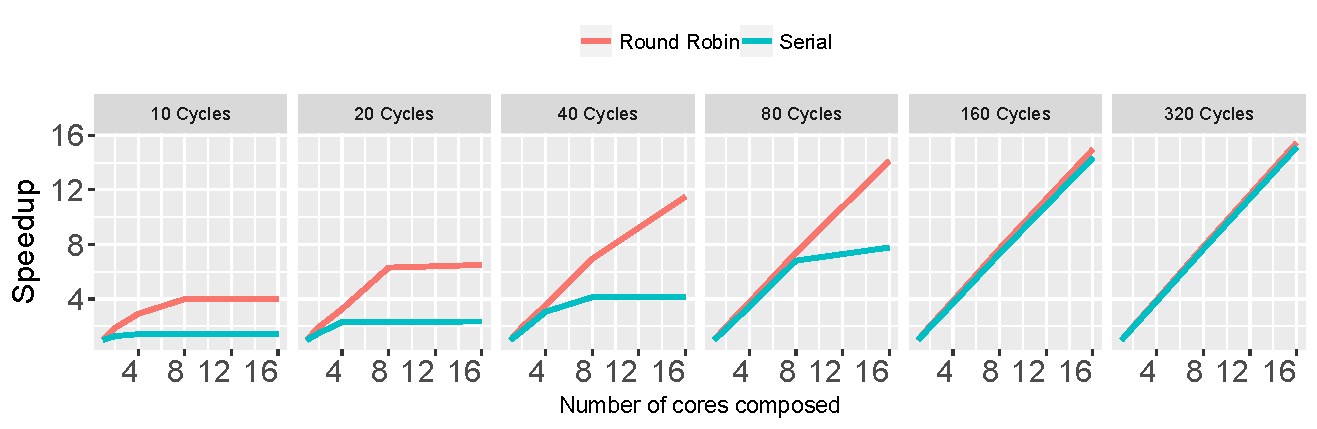
\includegraphics[width=1\textwidth]{chapter3/graphics/motivation_fetch.pdf}

    \caption{Speedup obtained through the old fetching technique and new fetching technique on a synthetic block with varying execution times (facet). Higher is better.}
    \label{fig:motivation_fetch}
	\vspace{1em}
\end{figure}

This section motivates the necessity of modifying the current fetching scheme and adding a value predictor to predict register dependencies to enable a higher amount of block level parallelism (BLP).

\subsection{Fetching mechanism}
Chapter~\ref{chp:cases} demonstrated how block size affects the performance of core composition, due to the fact that it increases the cost of synchronization and puts a strain on branch prediction.
Whilst the chapter focused on the size of blocks, it is not the sole determining factor of whether or not a set of blocks may be executed efficiently on a core composition.
For example, a small block containing load operations can potentially take at least 100 cycles to execute due to a cache miss.
In such a situation, the execution of the small block covers the latency caused by fetching multiple blocks on a large composition.
Thus, small blocks that take a long time to execute can benefit from core composition as long as the branch prediction is accurate.
Therefore, another feature to take into account when considering core composition is average execution time of a block.

The current core composition scheme (Chapter~\ref{chp:Background}), cores fetch in a serial fashion.
When a core composition is initiated, one of the cores will start fetching blocks until its instruction window is full.
Once the instruction window is full, the core will submit a fetch request to another core in the composition, which will then repreat the procedure.
However, if a block in the currently fetching core were to commit before the instruction window is full, the core will never submit a fetch request to another core.
In this situation, cores in a composition may remain inactive during the execution of a program.

Figure~\ref{fig:motivation_fetch} illustrates how a new fetching mechanism can improve the performance of core composition, especially on small blocks that can execute quickly.
The figure shows the speedup obtained via core composition when executing a synthetic block.
The synthetic block is only four instructions long using a custom instruction whose execution time is defined ahead of the simulation; these execution times are represented by the facets, and is executed 100000 times.
The reason a four instruction block was chosen is due to the fact that it allows for four blocks to be fetched on each core.
Recalling Chapter~\ref{chp:cases}, on average block-sizes were under 32 instructions long, thus each core needs to fetch four blocks before submitting a fetch request to another core.
The colours represent the different fetching schemes, "Old" being the fetching scheme described in more detail in Chapter~\ref{chp:Background} and used in Chapters~\ref{chp:streamit} and ~\ref{chp:cases}, whilst new defines the fetching mechanism which will be described in more detail later on.

In essence, the new fetching scheme aims to reduce the amount of communication between cores by allowing cores to fetch independently.
The results in the figure show that unless a block is at least 80 cycles long, it is difficult to efficiently use 16 core compositions using the normal fetching scheme.
To give a point of reference -- using data gathered from the SD-VBS benchmarks from Chapter~\ref{chp:cases} -- the average execution time of a block in SD-VBS is 20 cycles long.
However, with the new fetching scheme, 16 cores becomes useful when blocks are at least 40 cycles long, enabling a 3x speedup compared to the old fetching scheme.
For smaller core compositions, such as 2 and 4 fused cores, using a different fetching scheme from the traditional method allows for core composition to speedup execution when blocks are even 10 cycles long.

Overall, Figure~\ref{fig:motivation_fetch} demonstrates that the current fetching model is inadequate when blocks are small and execute quickly.
Whilst this was illustrated in previous chapters, this Section has demonstrated that modifying the fetching scheme can in fact improve the overall performance of core composition on blocks that were previously considered incompatible with core composition.

\subsection{Register dependencies}

In EDGE, global registers are only used for inter-block communication.
When multiple blocks are in flight, if a block requires to read a register that will be written to by an older block, it must naturally wait until that write has been execute.
Thus when executing multiple blocks in parallel data dependencies may arise.
This can be especially problematic when core composition is used, as up to 64 blocks could potentially be in flight at any moment.
If the data dependencies are not resolved quickly enough, then this causes blocks to execute in a serial fashion, which may erase any potential benefit from using the composition.

\lstset{
	backgroundcolor=\color{lbcolor},
	tabsize=2,
	rulecolor=,
	language=matlab,
        basicstyle=\tiny,
        upquote=true,
        aboveskip={1\baselineskip},
        columns=fixed,
        showstringspaces=false,
        extendedchars=true,
        breaklines=true,
        prebreak = \raisebox{0ex}[0ex][0ex]{\ensuremath{\hookleftarrow}},
        frame=single,
        showtabs=false,
        showspaces=false,
        showstringspaces=false,
        identifierstyle=\ttfamily,
        keywordstyle=\color[rgb]{0,0,1},
        commentstyle=\color[rgb]{0.133,0.545,0.133},
        stringstyle=\color[rgb]{0.627,0.126,0.941},
		numbers=left,
}

\begin{figure}[t]
\lstset{language=C,numbersep=4pt}
\begin{center}
\begin{lstlisting}
for(int i = 0; i < 1000; i++)
  for(int j = 0; j < 1000; j++)
         c[i][j] = a[i][j] * b[i][j];
\end{lstlisting}
\end{center}
\vspace{-1em}
\caption{Basic loop.}
\label{lst:bloop}
\vspace{1em}
\end{figure}

\begin{figure}[t]
    \centering
    
\includegraphics[width=1\textwidth]{chapter3/graphics/wip.pdf}

    \caption{Speedup of executing code in Listing~\ref{lst:bloop} using the new fetching mechanism, with and without value prediction. Higher is better.}
    \label{fig:motivation_reg}
	\vspace{1em}
\end{figure}

For example: Listing~\ref{lst:bloop} when unrolled should benefit from core composition.
The inner-most loop is compiled into a single block, with the iterators \textit{i} and \textit{j} being passed via register.
For small compositions, executing the code in Listing~\ref{lst:bloop} may improve the performance.
However for large compositions such as 8 or 16 cores, the register dependency may cause cores to have to wait on previous blocks to write to registers before being able to read the register value for their blocks.
In such a situation, large compositions should be able to execute faster than smaller compositions but the latency caused by register dependencies makes it impossible.

The register dependency issue is a common problem for superscalar processors~\cite{} where ILP is limited by data-dependencies.
One solution to the problem of data-dependencies is adding a value predictor to the processor.
To summarize Section~\ref{} of Chapter~\ref{chp:Background}, value predictors predict data at specific addresses, in a similar fashion to branch predictors.
This allows instructions to execute with speculative data, and thus decrease the penalty caused by data-dependencies.
In cases where data is modified in a regular way, value predictors 
Whilst the register dependencies found in Listing~\ref{lst:bloop} are problematic, they can be resolved through the use of a value predictor.

Figure~\ref{fig:motivation_reg} shows the performance of executing the code in Listing~\ref{lst:bloop} with and without value prediction on different core compositions using the new fetching scheme.
The speedup is obtained by comparing the execution time of core compositions to a single core.
The figure shows that without value prediction the higher core compositions do not perform much better than the smaller compositions; once again due to the latencies caused by data-dependencies.
Using a value predictor (shown in red) unlocks the speedup potential of large compositions.
